\documentclass[12pt]{article} % use larger type; default would be 10pt
\usepackage[utf8]{inputenc} % set input encoding (not needed with XeLaTeX)

%%% PAGE DIMENSIONS
\usepackage{geometry} % to change the page dimensions
\geometry{a4paper} % or letterpaper (US) or a5paper or....
\geometry{margin=2cm} % or letterpaper (US) or a5paper or....

\usepackage{graphicx} % support the \includegraphics command and options
\usepackage[parfill]{parskip} % Activate to begin paragraphs with an empty line rather than an indent
\usepackage{times} % for Times Roman default font

%%% PACKAGES
\usepackage{booktabs} % for much better looking tables
\usepackage{array} % for better arrays (eg matrices) in maths
\usepackage{paralist} % very flexible & customisable lists (eg. enumerate/itemize, etc.)
\usepackage{verbatim} % adds environment for commenting out blocks of text & for better verbatim
\usepackage{subfig} % make it possible to include more than one captioned figure/table in a single float

%%% HEADERS & FOOTERS
\usepackage{fancyhdr} % This should be set AFTER setting up the page geometry
\pagestyle{fancy} % options: empty , plain , fancy
\renewcommand{\headrulewidth}{0pt} % customise the layout...
\lhead{}\chead{}\rhead{}
\lfoot{}\cfoot{\thepage}\rfoot{}

\makeatletter
\renewcommand{\maketitle}{%
  {\bfseries{\scshape{\Large{\@title\par}}}}
}
\makeatother

\hyphenation{Kiwi-bank} % otherwise it may get hyphenated as Ki-wibank

%%% END Article customizations

%%% The "real" document content comes below...

\title{Mt Mantell: 15 November 2018}

\begin{document}
  \maketitle

We'd heard there was a track leading up Mt Mantell from the Maruia Saddle road.  It starts about 300m beyond the fifth ford from home (or 300m before the second ford if coming from Murchison).  From the road one can see an orange track marker on a fairly large beech tree, if one looks hard enough.  It is a bit of a scramble getting off the road though.  The track follows the ridge on which high point 680 is located.

We started walking about 09:15 and got to the bush line (at about 1310m) at about 11:30; i.e., we'd climbed about 885m in 2$\frac{1}{4}$ hours.  Most of the track is pretty steep, although there is a welcome flattish section of about half a kilometre around 650m.  Although the track markers are a bit sparse, we did not find the track difficult to follow.  Indeed the bush was very open (we saw a couple of goats so that could have something to do with it).

We lunched at high point 1472, from which the photographs were taken.  At 12:30 we headed off towards the knob further along the ridge (it's not labelled but is about 1482m).  At this point I went ahead as Robyn had decided not to go all the way.  It took me about 45 minutes to reach the summit from the lunch spot.  I followed the ridge all the way, although some of the sections were pretty steep especially towards the end.  On returning I headed ENE off Mt Mantell for a short way before dropping off and sidling to miss the steeper sections.  I also sidled around the knob that Robyn had gone to. I caught Robyn about 1100-1000m and we finished the trip together.

\begin{figure}[ht]
%\centering
\begin{minipage}{.5\linewidth}
\begin{flushleft}
   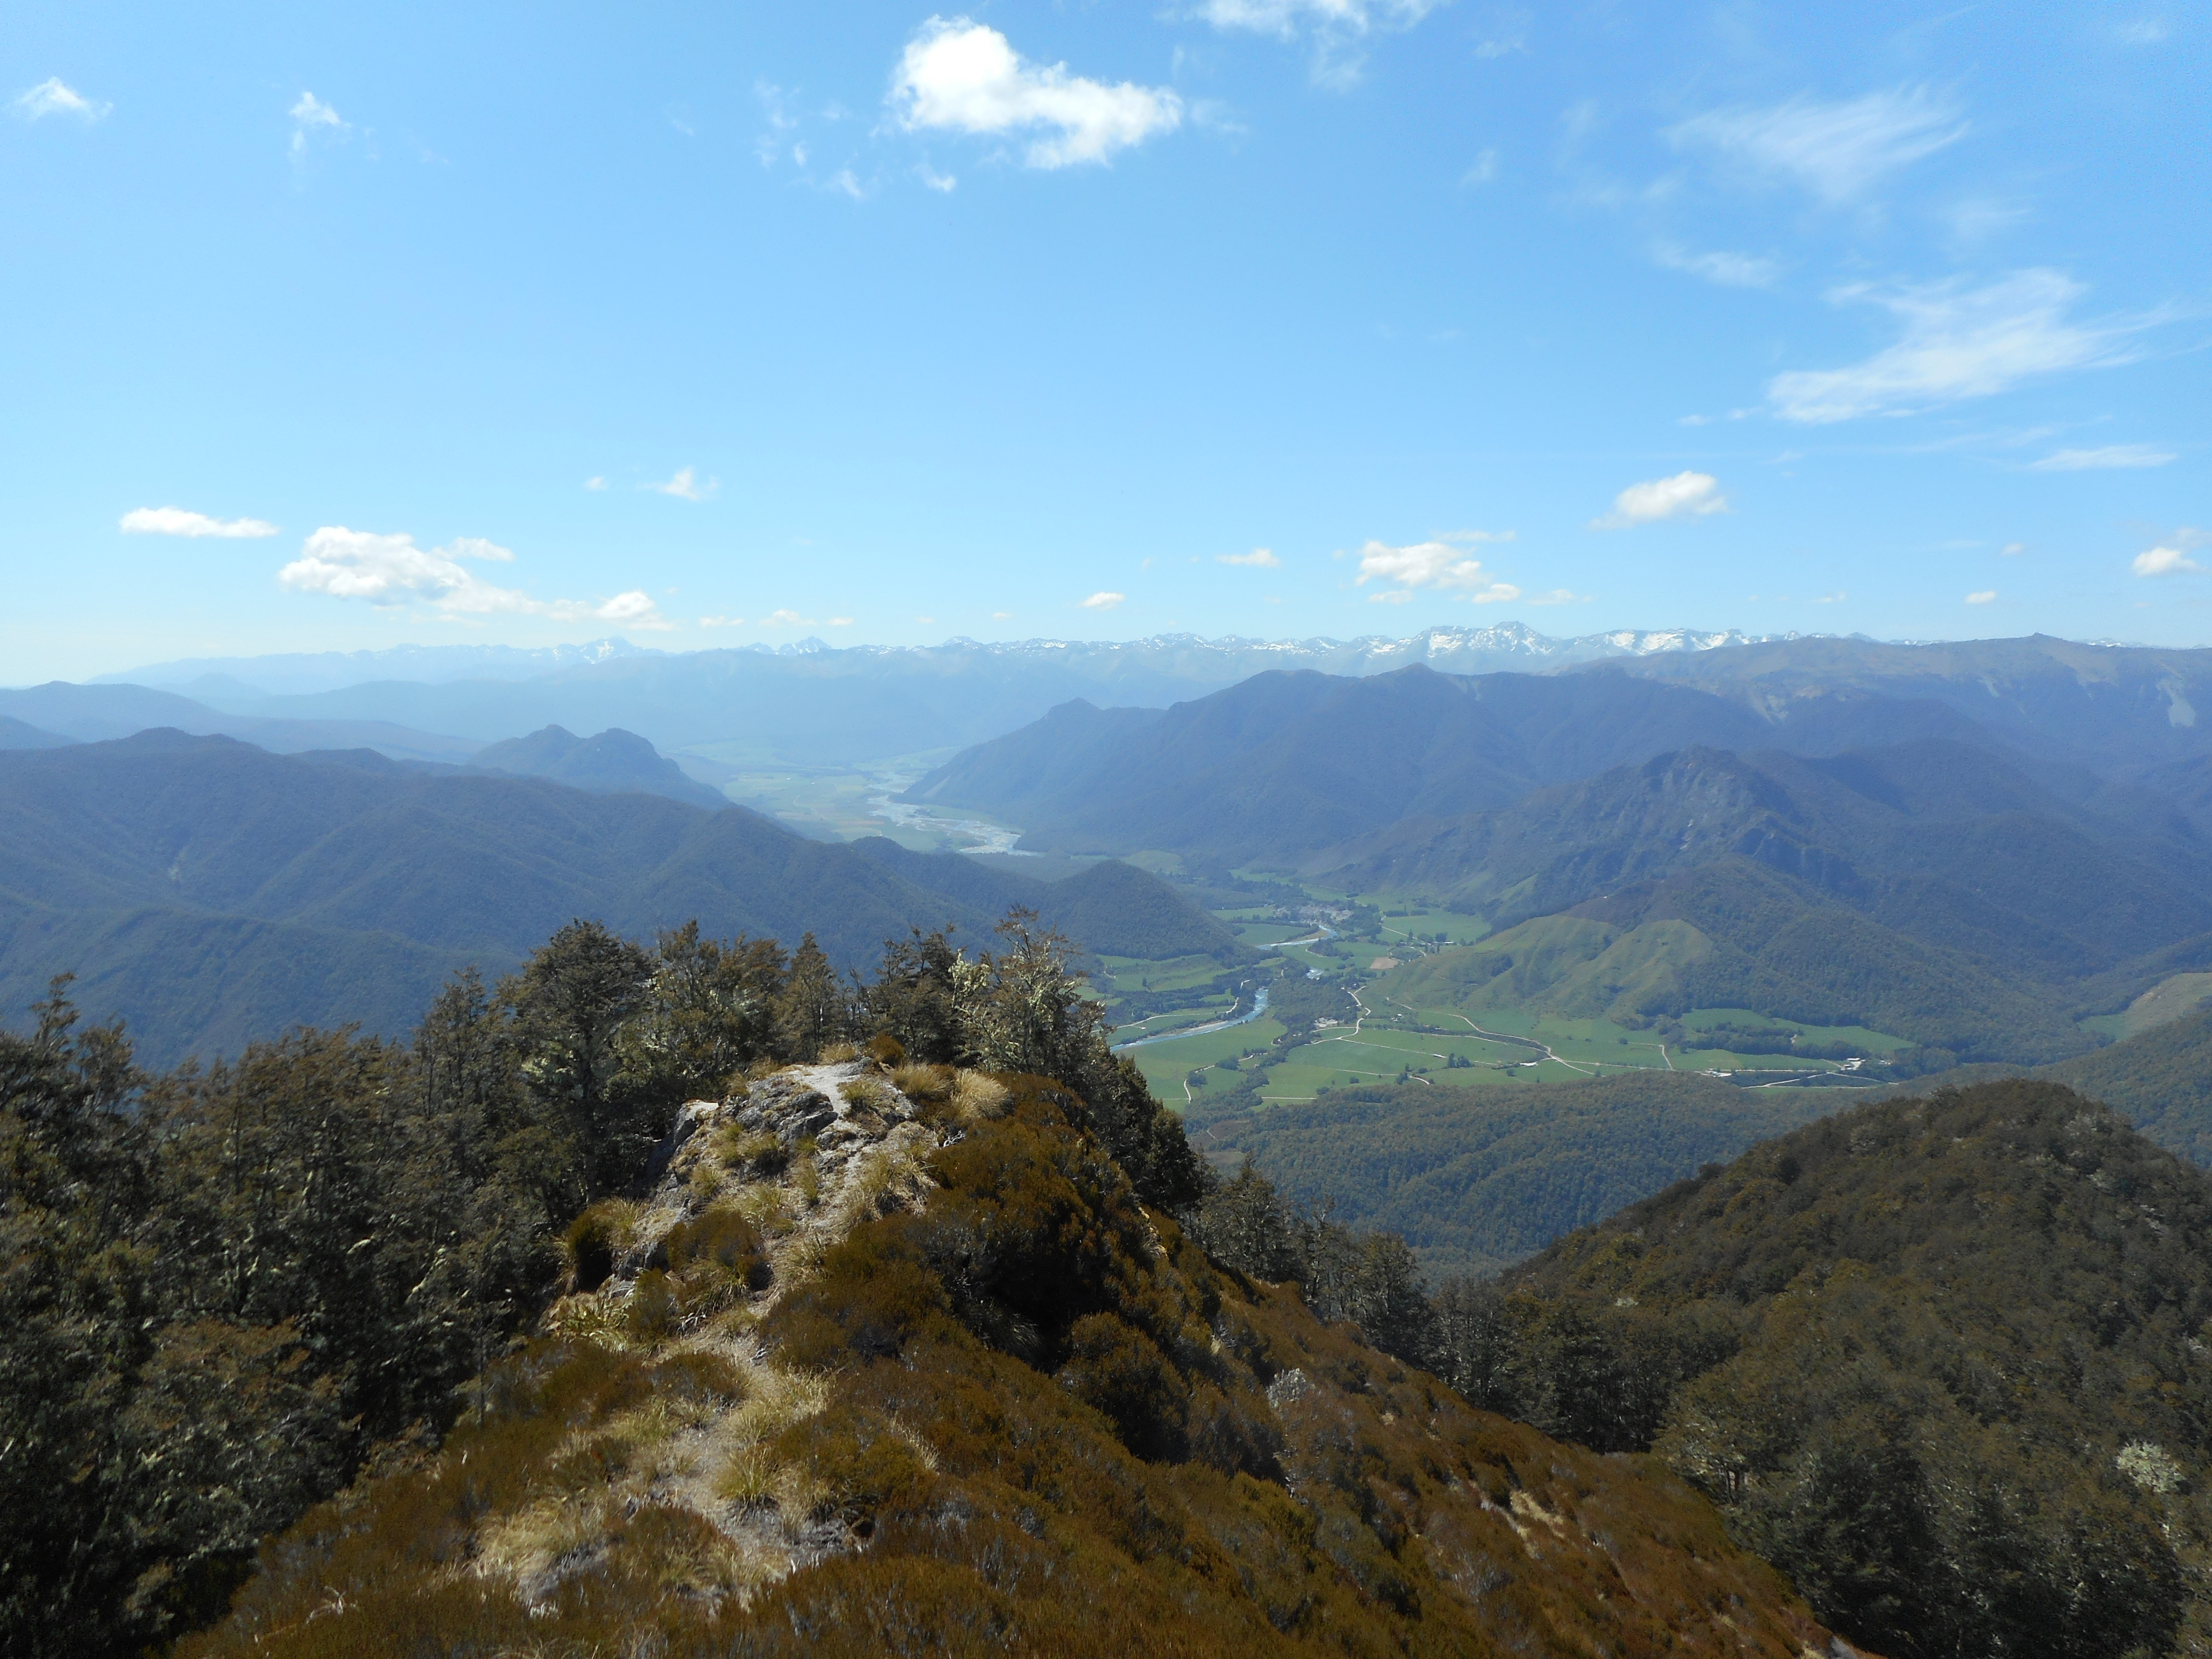
\includegraphics[width=8.5cm]{MtMantell15Nov2018Photo1}
   \captionof{figure}{View towards home}
\end{flushleft}
\end{minipage}
\begin{minipage}{.5\linewidth}
\begin{flushright}
    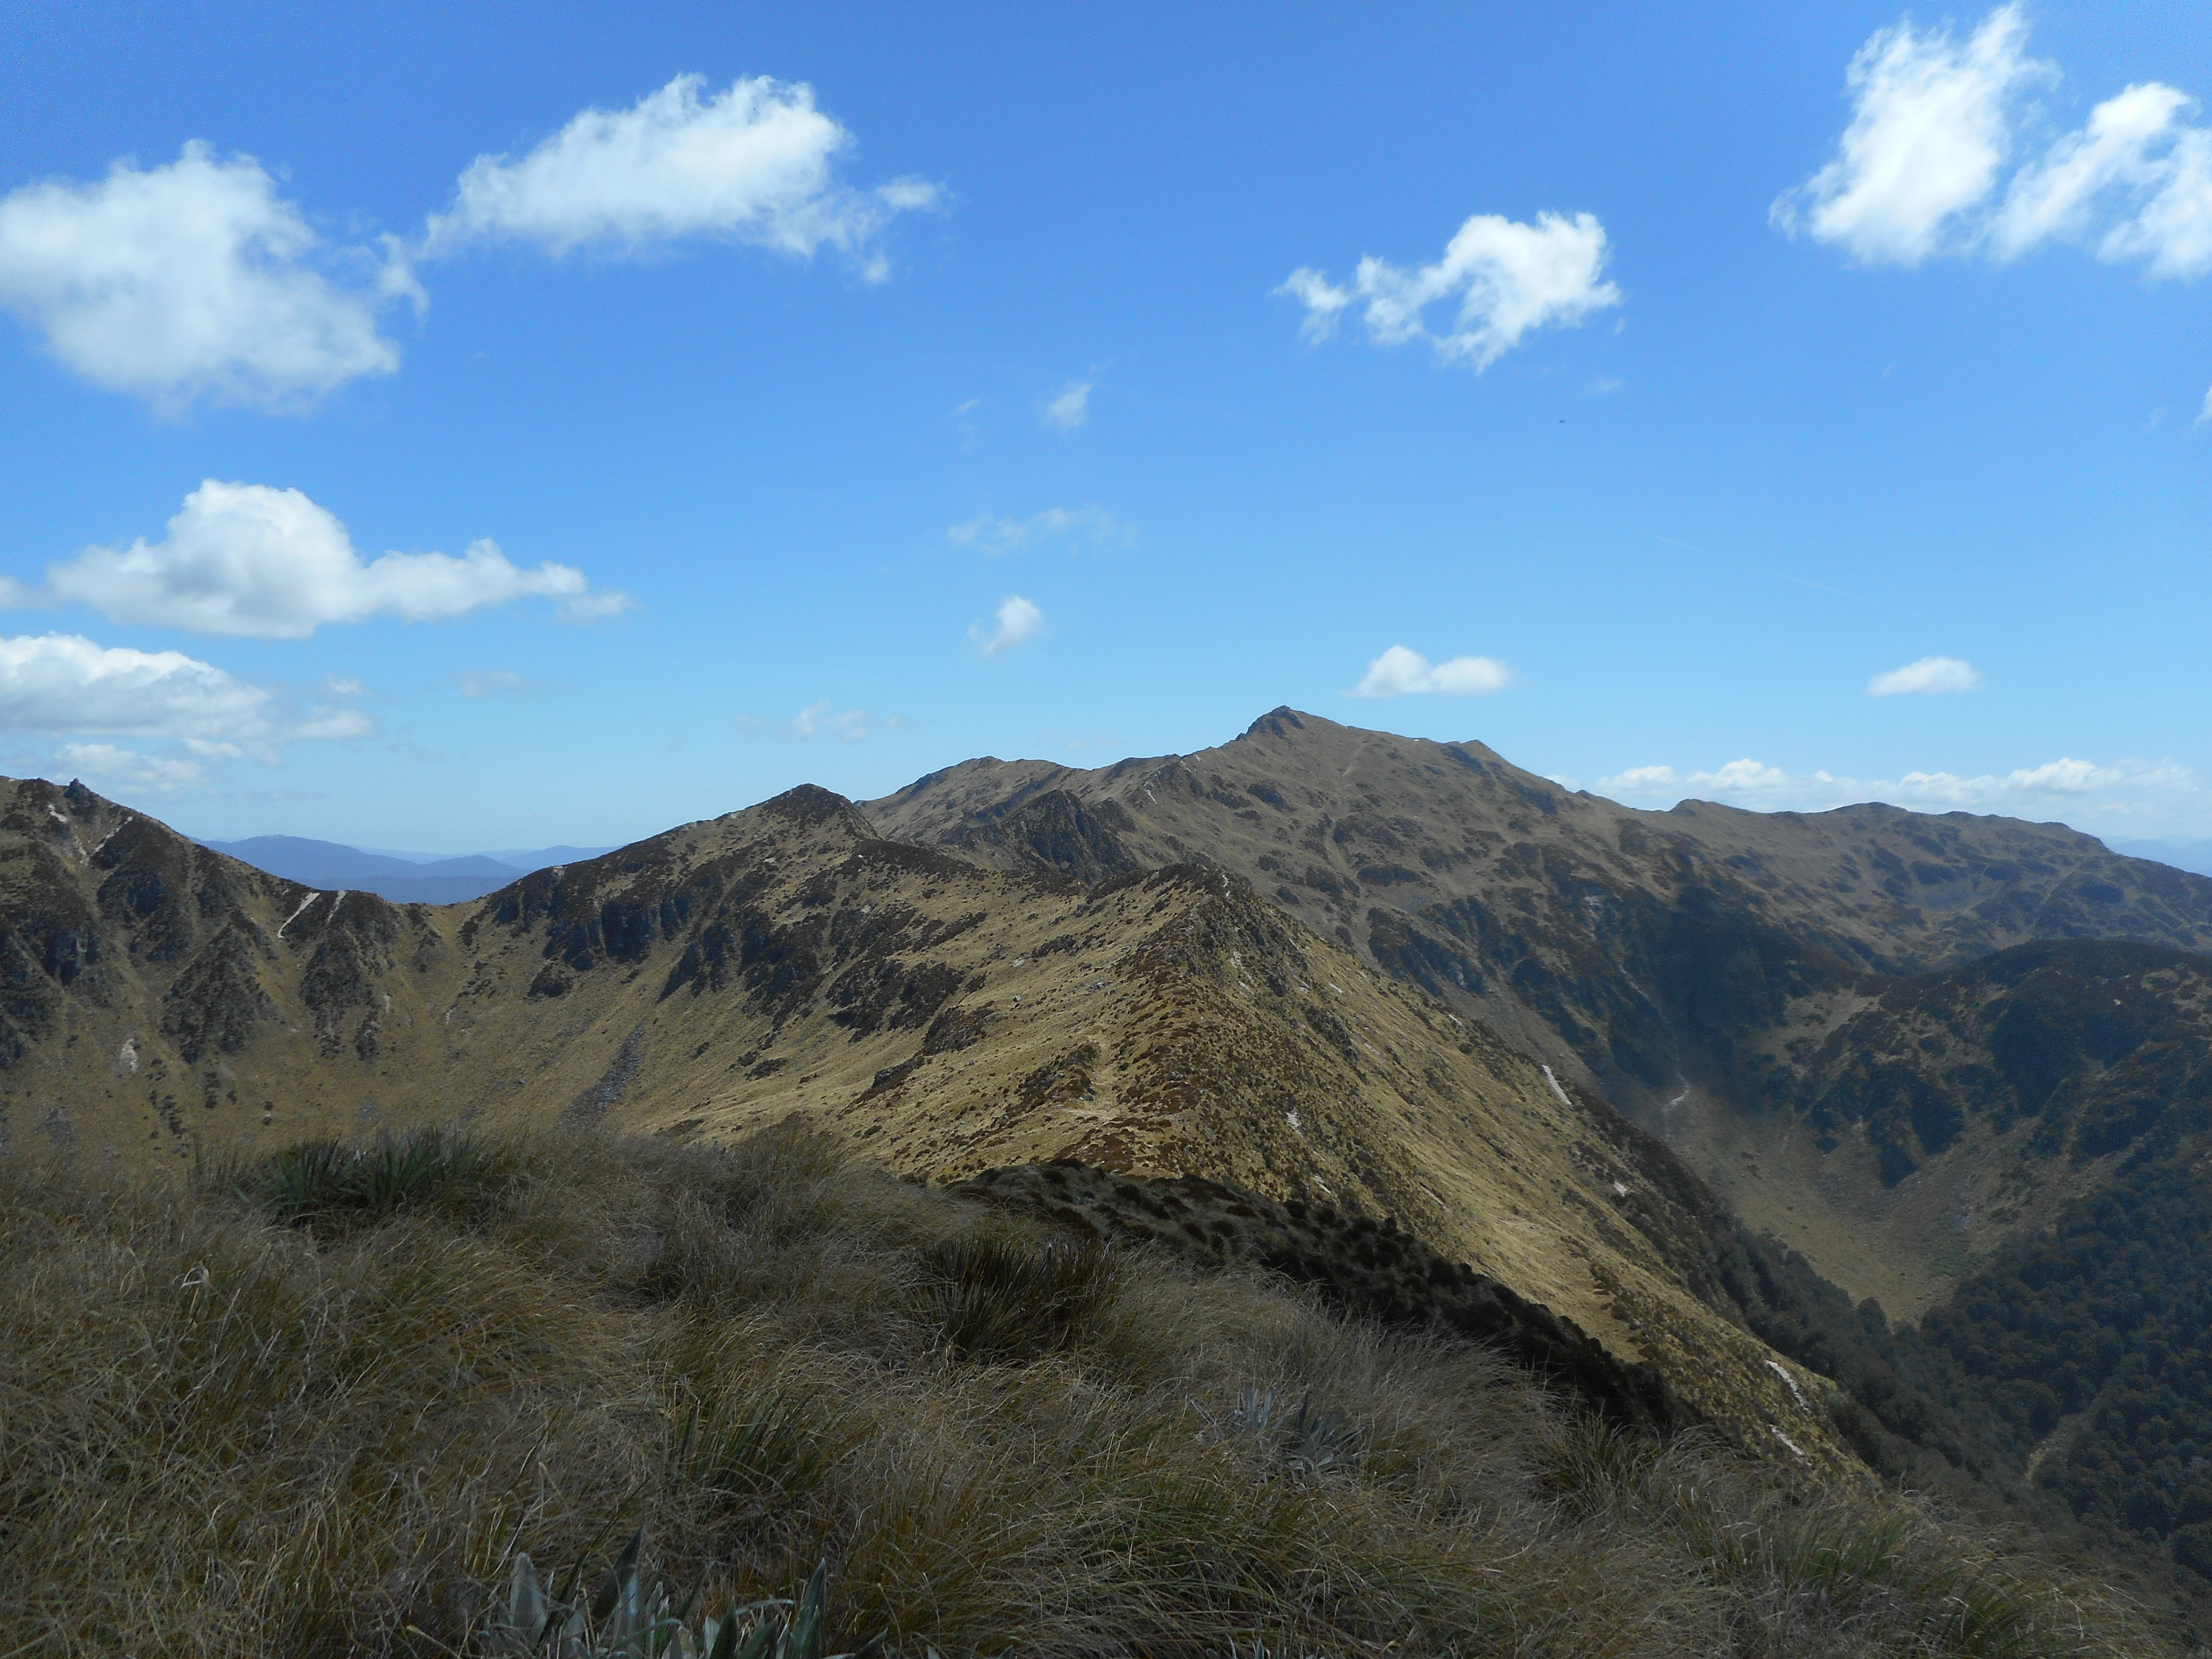
\includegraphics[width=8.5cm]{MtMantell15Nov2018Photo2}
    \captionof{figure}{Mt Mantell from high point 1472}
\end{flushright}
\end{minipage}
\end{figure}

We arrived back at the car around 15:25; i.e., six and a bit hours after leaving.

\begin{flushright}
Robyn, Peter and dog
\end{flushright}

\end{document}
